\documentclass[a4paper,10pt]{article}

% Hier die Nummer des Blatts und Autoren angeben.
\newcommand{\blatt}{1}
\newcommand{\autor}{Alexander Hildebrandt}

\usepackage{hci}

\begin{document}
% Seitenkopf mit Informationen
\kopf
\renewcommand{\figurename}{Figure}

\aufgabe{1}
\begin{enumerate}

\item Um die Navigation der Inuit erleichtern zu können, muss das Produkt kaelteresistent sein. Da es wahrscheinlich keine feste Stromquelle auf den Schiffen geben wird, muss das Produkt mit Batterien betrieben werden. Es ist anzunehmen, dass die Zielgruppe nicht unbedingt Technik-affin ist. Deshalb muss die Bedienung des Produktes sehr simpel gehalten werden und statt Blick auf viele kleine Features, kann das Produkt eher auf wenige Core-Features beschraenkt sein. Auszerdem waere ein wasserfestes, nicht sinkendes Gehaeuse eine sinnvolle Erweiterung.

\item Skizze:

\begin{figure}[ht]
\centering 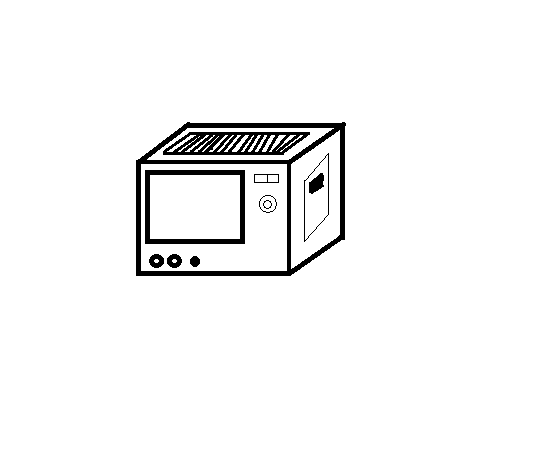
\includegraphics[width=0.4\textwidth]{images/produkt.png}
\end{figure}

\item Das Produkt verfuegt an der Front ueber einen Bildschirm, um eine Satellitenkarte der Umgebung anzuzeigen. Per GPS ist der Nutzer in der Karte markiert. Unter dem Bildschirm sind zwei Drehschalter, die die Karte bewegen. Es gibt keinen Touchscreen, da die Inuit Handschuhe tragen, wodurch sich ein Touchscreen nicht lohnen wuerde. Des Weiteren gibt es einen Knopf, mit dem man eine neue Markierung in die Karte setzen kann, um wichtige Punkte wiederzufinden. Rechts neben dem Bildschirm ist ein Schalter, um das Gerät ein- und auszuschalten. Darunter befindet sich ein weiterer Drehschalter, der die Helligkeit des Bildschirmes bestimmt. Da die Inuit lange Strecken ohne Stromquelle im Boot zuruecklegen muessen, wird sich die Stromsparende Funktion der Helligkeitseinstellung lohnen. Oben auf dem Gerät ist eine Platte, um Solarenergie einzufangen. Da die Sonneneinstrahlung von der Jahreszeit abhaengt und das halbe Jahr lang so gut wie keine Sonne so weit im Norden sein wird, muss man auf Batterien zurueckgreifen, die sich an der Seite des Geraetes einfuehren lassen. Die Huelle ist mit wasserfestem Plastik ueberzogen. Im Inneren ist so viel Aluminium wie möglich verbaut, um das Gewicht zu reduzieren, sodass das Geraet nicht im Wasser sinkt. 

\end{enumerate}

\end{document}
